\section{Module de curiosité appliqué au contrôle}
\begin{frame}{Nécessité d'exploration d'un environnement}

    Nécessité d'exploration de l'environnement ?

\begin{columns}[T] % align columns
\begin{column}{.48\textwidth}
\begin{center}
    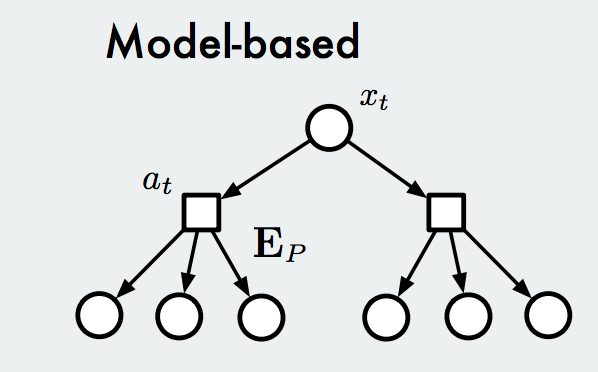
\includegraphics[scale=.24]{./curiosity/1}
\end{center}
\end{column}%
\hfill%
\begin{column}{.58\textwidth}
\begin{itemize}
    \item \vip{Dynamique de l'environnement}\\$\rightarrow$ Connue \\ $\rightarrow$ Fonction d'état-action: Connue \\ $\rightarrow$ Politique: Connue
\end{itemize}

\begin{center}
    \bigskip
    
\includegraphics[scale=.3]{./curiosity/3}
\end{center}

\end{column}%
\end{columns}


\end{frame}

\begin{frame}{Nécessité d'exploration d'un environnement}

    Nécessité d'exploration de l'environnement ?

\begin{columns}[T] % align columns
\begin{column}{.48\textwidth}
\begin{center}
    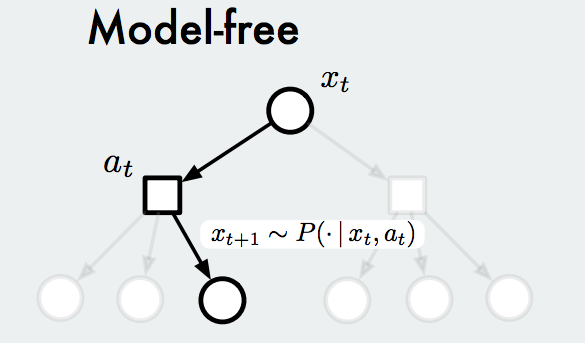
\includegraphics[scale=.24]{./curiosity/2}
\end{center}
\end{column}%
\hfill%
\begin{column}{.58\textwidth}
\begin{itemize}
    \item \vip{Dynamique de l'environnement}\\$\rightarrow$ Inconnue \\ $\rightarrow\:$ Fonction d'état-action: Inconnue \\ $\rightarrow\:$ Politique: Inconnue
\end{itemize}

\begin{center}
    
\includegraphics[scale=.3]{./curiosity/3}
\end{center}

\end{column}%
\end{columns}


\end{frame}
